\documentclass[12pt]{article}

% a template that a friend gave, it's worked well enough for me
% i have added some packages and stuff that have proved useful

\usepackage{fancyhdr}
\usepackage{tipa}
\usepackage{fontspec}
\usepackage{amsfonts}
\usepackage{enumitem}
\usepackage[margin=1in]{geometry}
\usepackage{graphicx}
\usepackage{float}
\usepackage{amsmath}
\usepackage{braket}
\usepackage{amssymb}
\usepackage{booktabs}
\usepackage{hyperref}
\usepackage{mathtools}
\usepackage{xcolor}
\usepackage{float}
\usepackage{algpseudocodex}
\usepackage{titlesec}
\usepackage{bbm}

\pagestyle{fancy}
\fancyhf{} % sets both header and footer to nothing
\lhead{Kevin Sheng}
\setmainfont{Comic Neue}
\renewcommand{\headrulewidth}{1pt}
\setlength{\headheight}{0.75in}
\setlength{\oddsidemargin}{0in}
\setlength{\evensidemargin}{0in}
\setlength{\voffset}{-.5in}
\setlength{\headsep}{10pt}
\setlength{\textwidth}{6.5in}
\setlength{\headwidth}{6.5in}
\setlength{\textheight}{8in}
\renewcommand{\headrulewidth}{0.5pt}
\renewcommand{\footrulewidth}{0.3pt}
\setlength{\textwidth}{6.5in}
\usepackage{setspace}
\usepackage{multicol}
\usepackage{float}
\setlength{\columnsep}{1cm}
\setlength\parindent{24pt}
\usepackage [english]{babel}
\usepackage [autostyle, english = american]{csquotes}
\MakeOuterQuote{"}

\setlength{\parskip}{6pt}
\setlength{\parindent}{0pt}

\titlespacing\section{0pt}{12pt plus 4pt minus 2pt}{0pt plus 2pt minus 2pt}
\titlespacing\subsection{0pt}{12pt plus 4pt minus 2pt}{0pt plus 2pt minus 2pt}
\titlespacing\subsubsection{0pt}{12pt plus 4pt minus 2pt}{0pt plus 2pt minus 2pt}

\hypersetup{colorlinks=true, urlcolor=blue}

\newcommand{\correction}[1]{\textcolor{red}{#1}}


\rhead{ECE 102}

\newcommand{\rect}{\operatorname{rect}}

\begin{document}

\begin{enumerate}
      \item \begin{enumerate}
                  \item The given formula is exactly what the system does.
                        It multiplies $x(t)$ with $e^t$, convolves it with $h(t)$,
                        and finally multiplies that with $e^{-t}$.
                  \item \[\begin{aligned}
                                    y(t)
                                     & = \int_{-\infty}^{\infty} e^{t-\tau} x(t-\tau) h(\tau)\,dt \cdot e^{-t} \\
                                     & = \int_{-\infty}^{\infty} x(t-\tau) e^{-\tau} h(\tau)\,dt               \\
                                     & = \int_{-\infty}^{\infty} x(t-\tau) h'(\tau)\,dt\quad\square
                              \end{aligned}\]
                  \item $y(t)=(h' * x)(t)$, so the combined system is LTI
                        since convolution is inherently LTI.
                        The impulse response of this system was already derived in the previous question:
                        \[h'(t)=e^{-t}h(t)\]
            \end{enumerate}
      \item \begin{enumerate}
                  \item $f(t)$ isn't an eigenfunction.
                        \begin{align*}
                              (f * h)(t)
                               & = \int_{-\infty}^{\infty} (t-\tau) \cdot h(\tau)\,d\tau                                        \\
                               & = \int_{-\infty}^{\infty} t \cdot h(\tau)-\tau \cdot h(\tau)\,d\tau                            \\
                               & = t \int_{-\infty}^{\infty} h(\tau)\,d\tau - \int_{-\infty}^{\infty} \tau \cdot h(\tau)\,d\tau \\
                               & \ne \alpha \cdot t
                        \end{align*}
                  \item $f(t)$ isn't an eigenfunction.
                        \begin{align*}
                              (f * h)(t)
                               & = \int_{-\infty}^{\infty} e^{j\omega(t-\tau)} u(t-\tau) h(\tau)\,d\tau             \\
                               & = e^{j \omega t} \int_{-\infty}^{\infty} e^{-j\omega\tau} u(t-\tau) h(\tau)\,d\tau \\
                               & = e^{j \omega t} \int_{-\infty}^{\infty} u(t-\tau) h'(\tau)\,d\tau
                               & \text{where }h'(\tau)=h(\tau)e^{-j\omega\tau}                                      \\
                               & = e^{j\omega t} (u * h')(t)                                                        \\
                               & \ne \alpha \cdot e^{j\omega t} u(t)
                        \end{align*}
            \end{enumerate}
      \item \begin{enumerate}
                  \item \begin{enumerate}
                              \item
                        \end{enumerate}
                  \item \begin{enumerate}
                              \item $z_k=3x_k+2y_k$
                              \item \[w_k=\begin{cases}
                                                y_k           & k \equiv 1 \pmod 2 \\
                                                x_{k/2} + y_k & k \equiv 0 \pmod 2
                                          \end{cases}\]
                        \end{enumerate}
            \end{enumerate}
      \item \begin{enumerate}
                  \item \begin{enumerate}
                              \item \[g(t)=\sum_{k=-\infty}^{\infty} (3c_k)e^{jk\omega_0t}\]
                              \item \[g(t)=\sum_{k=-\infty}^{\infty} c_{-k}e^{jk\omega_0at}\]
                              \item \[\begin{aligned}
                                                g(t)
                                                 & = \sum_{k=-\infty}^{\infty} c_k e^{jk\omega_0(t-t_0)}                                         \\
                                                 & = \sum_{k=-\infty}^{\infty} c_k e^{jk\omega_0t}e^{-jk\omega_0t_0}                             \\
                                                 & = \boxed{\sum_{k=-\infty}^{\infty} \left(c_k \cdot e^{-jk\omega_0t_0}\right) e^{jk\omega_0t}}
                                          \end{aligned}\]
                        \end{enumerate}
                  \item \begin{itemize}
                              \item $x_1(t)$ is even.
                                    \begin{align*}
                                          x_1(-t)
                                           & = \sum_{k=-100}^{100} \cos(k\pi)\exp\left(-jk\frac{2\pi}{50}t\right) \\
                                           & = \sum_{k=-100}^{100} \cos(-k\pi)\exp\left(jk\frac{2\pi}{50}t\right) \\
                                           & = \sum_{k=-100}^{100} \cos(k\pi)\exp\left(jk\frac{2\pi}{50}t\right)  \\
                                           & = x_1(t)
                                    \end{align*}
                              \item $x_2(t)$ isn't even. It \textit{is} odd, however.
                                    \begin{align*}
                                          x_2(-t)
                                           & = \sum_{k=-100}^{100} j\sin\left(\frac{k\pi}{2}\right)\exp\left(-jk\frac{2\pi}{50}t\right) \\
                                           & = \sum_{k=-100}^{100} j\sin\left(-\frac{k\pi}{2}\right)\exp\left(jk\frac{2\pi}{50}t\right) \\
                                           & = \sum_{k=-100}^{100} -j\sin\left(\frac{k\pi}{2}\right)\exp\left(jk\frac{2\pi}{50}t\right) \\
                                           & = -x_2(t)
                                    \end{align*}
                        \end{itemize}
                  \item \begin{enumerate}
                              \item 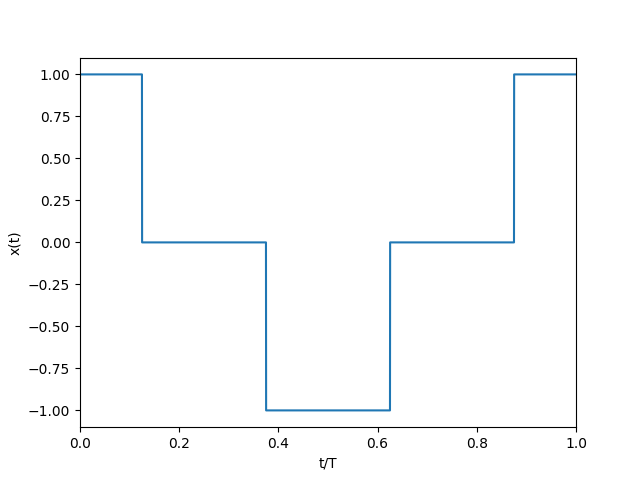
\includegraphics[width=12cm]{img/hw4/even}
                              \item 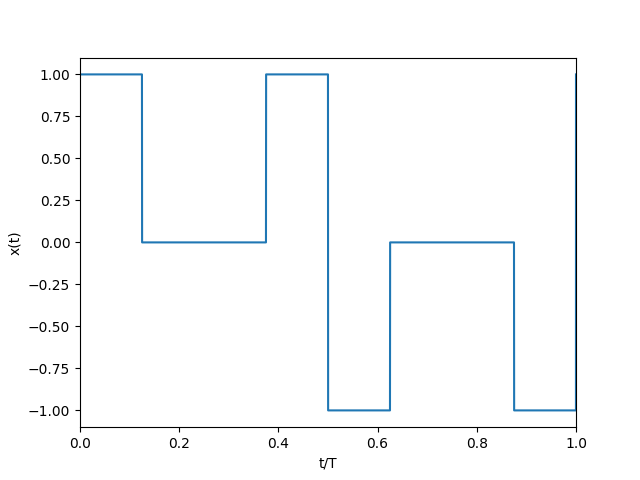
\includegraphics[width=12cm]{img/hw4/odd}
                        \end{enumerate}
            \end{enumerate}
      \item After this PDF will be the Jupyter Notebook I ran.
\end{enumerate}
\end{document}
